% Generated by thesis/ch7/exp2/networks.py -- do not edit by hand.
\begin{sidewaysfigure}
  \centering
  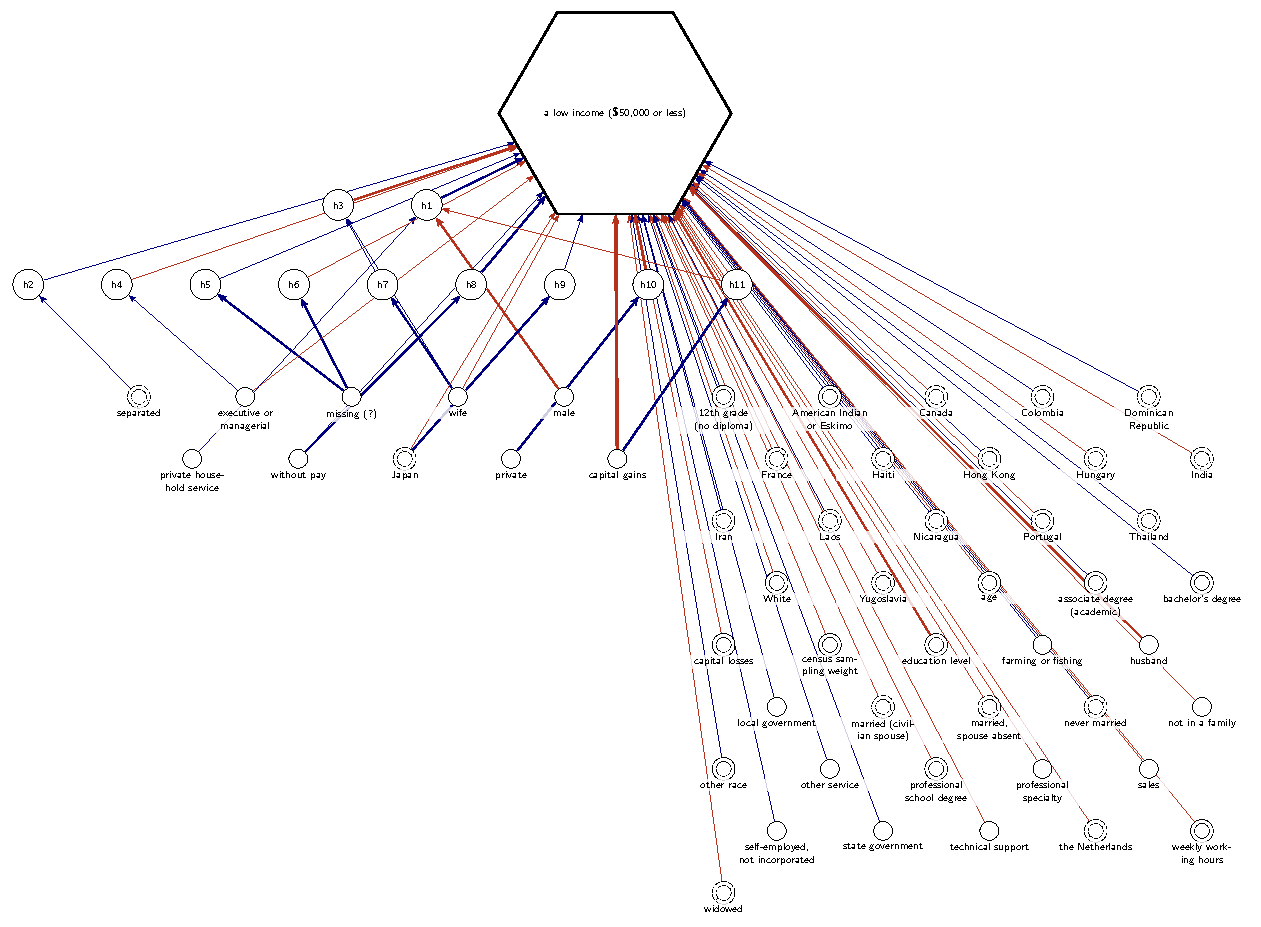
\includegraphics[width=\textheight,height=0.78\textwidth,keepaspectratio]{figures/exp2/networks/adult-s0-raw}
  \caption{Adult, seed 0 (adult-s0): the network as trained, before any explanation, in full. Inputs at the bottom (every input column its own node), hidden units by depth, the output at the top; 51 of 107 input columns are connected, with 11 hidden units and 70 enabled connections. Blue: positive weight (raises the score); red: negative weight (lowers it); thicker: larger weight. Orange outline and up arrow: raises the final prediction; teal and down arrow: lowers it; grey and double arrow: depends. Not used (no connection; 56 columns): federal government, never worked, self-employed, incorporated, 10th grade, 11th grade, doctorate, high-school graduate, master's degree, preschool, some college, 1st-4th grade, 5th-6th grade, 7th-8th grade, 9th grade, associate degree (vocational), divorced, married to a member of the armed forces, missing (?), administrative or clerical, protective service, transport or moving, armed forces, craft or repair, handlers or cleaners, machine operator or inspector, other relative, own child, unmarried, Asian or Pacific Islander, Black, missing (?), Cambodia, Germany, Greece, Guatemala, Honduras, Ireland, Italy, Jamaica, Mexico, outlying US territories (Guam, US Virgin Islands), Peru, China, the Philippines, Poland, Puerto Rico, Scotland, 'South' (as recorded), Taiwan, Trinidad and Tobago, the United States, Vietnam, Cuba, Ecuador, El Salvador and England.}
  \label{fig:exp2-net-adult-s0-raw}
\end{sidewaysfigure}
